\documentclass[11pt]{article}
\usepackage{../stat110}
\usepackage{graphicx}
\usepackage{epigraph}
\usepackage{hyperref}

%\STAFF

\begin{document}

\SectionNotes{11}{Markov Chains, Monte Carlo and Limit Theorems}{Luis Perez (luisperez@college.harvard.edu)}{Aidi Zhang (aidizhang@college.harvard.edu)}


\setlength{\epigraphwidth}{.6\textwidth}
\epigraph{A man in daily muddy contact with field experiments could not be expected to have much faith in any direct assumption of independently distributed normal errors.}{George Box}

\section*{Administrivia}
Section notes modified from William and Sebastian.

\section*{Law of Large Numbers (LLN)}
Let us have $X_1, X_2, X_3 \dots$ be i.i.d.. We define $\bar{X}_n = \frac{X_1 + X_2 + X_3 + \dots + X_n}{n}$ The Law of Large Numbers states that as $n \longrightarrow \infty$, $\bar{X}_n \longrightarrow E(X)$.

\section*{Central Limit Theorem (CLT)}
\subsection*{Approximation using CLT}
We use $\dot{\,\sim\,}$ to denote \emph{is approximately distributed}. {We can use the central limit theorem when we have a random variable, $Y$ that is a sum of $n$ i.i.d. random variables with $n$ large. Let us say that $E(Y) = \mu_Y$ and $\var(Y) = \sigma^2_Y$. We have that:
\[Y \dot{\,\sim\,} \N(\mu_Y, \sigma^2_Y)\]

When we use central limit theorem to estimate $Y$, we usually have $Y = X_1 + X_2 + \dots + X_n$ or $Y = \bar{X}_n= \frac{1}{n}(X_1 + X_2 + \dots + X_n)$. Specifically, if we say that each of the $X_i$ have mean $\mu_X$ and $\sigma^2_X$, then we have the following approximations.

\[ X_1 + X_2 + \dots + X_n \dot{\,\sim\,} \N(n\mu_X, n\sigma^2_X) \]
\[ \bar{X}_n = \frac{1}{n}(X_1 + X_2 + \dots + X_n) \dot{\,\sim\,} \N(\mu_X, \frac{\sigma^2_X}{n}) \]


\subsection*{Asymptotic Distributions using CLT}

We use $\xrightarrow{d}$ to denote \emph{converges in distribution to} as $n \longrightarrow \infty$. These are the same results as the previous section, only letting $n \longrightarrow \infty$ and not letting our normal distribution have any $n$ terms.
\[\frac{1}{\sigma\sqrt{n}} (X_1 + \dots + X_n - n\mu_X) \xrightarrow{d} \N(0, 1)\]
\[\frac{\bar{X}_n - \mu_X}{\sfrac{\sigma}{\sqrt{n}}} \xrightarrow{d} \N(0, 1)\]

\subsection*{Intuitive Explanation}
\url{https://www.quora.com/What-is-an-intuitive-explanation-of-the-Central-Limit-Theorem}

\section*{Continuity Correction}
If we have $X$ discrete on integers with mean $\mu_X$ and variance $\sigma^2_X$, with $X$ being the sum of many things (which validates the use of CLT), then we can approximate $X$ as $Y \sim \N(\mu_X, \sigma^2_X)$. To approximate the probability that $X = k$, we apply the continuity correction.
\[P(X = k) \approx P( k - \frac{1}{2} \leq Y \leq k + \frac{1}{2})\]
Thus we can approximate this probability $P(X = k)$ with the following:
\[P(X = k) \approx P\left( \frac{k - \frac{1}{2} - \mu_X}{\sigma_X} \leq \frac{Y - \mu_X}{\sigma_X} \leq \frac{k + \frac{1}{2} - \mu_X}{\sigma_X}\right) = \Phi\left(\frac{k + \frac{1}{2} - \mu_X}{\sigma_X} \right) - \Phi\left( \frac{k - \frac{1}{2} - \mu_X}{\sigma_X} \right)\]
We can also use continuity correction to estimate the CDF.
\[P(X \leq k) \approx P\left(Y \leq k + \frac{1}{2}\right)\]



\section*{Definition}
A Markov Chain is a walk along a (finite or infinite, but for this class usually finite) discrete \textbf{state space} \{1, 2, \dots, M\}. We let $X_t$ denote which element of the state space the walk is on at time $t$. The Markov Chain is the set of random variables denoting where the walk is at all points in time, $\{X_0, X_1, X_2, \dots \}$, as long as if you want to predict where the chain is at at a future time, you only need to use the present state, and not any past information. In other words, the \emph{given the present, the future and past are conditionally independent}. Intuitive Explanation - \url{http://qr.ae/GYFJO}. Formal Definition:
\[P(X_{n+1} = j | X_0 = i_0, X_1 = i_1, \dots, X_n = i) = P(X_{n+1} = j | X_n = i)\]
\section*{State Properties}
A state is either recurrent or transient.
\begin{itemize}
\item If you start at a \textbf{Recurrent State}, then you will always return back to that state at some point in the future.  \textmusicalnote \emph{You can check-out any time you like, but you can never leave.}  \textmusicalnote
\item Otherwise you are at a \textbf{Transient State}. There is some probability that once you leave you will never return. \textmusicalnote \emph{You don't have to go home, but you can't stay here.} \textmusicalnote
\end{itemize}
A state is either periodic or aperiodic.
\begin{itemize}
\item If you start at a \textbf{Periodic State} of period $k$, then the GCD of all of the possible number steps it would take to return back is  $> 1$.
\item Otherwise you are at an \textbf{Aperiodic State.} The GCD of all of the possible number of steps it would take to return back is 1.
\end{itemize}


\section*{Transition Matrix}
Element $q_{ij}$ in square transition matrix Q is the probability that the chain goes from state $i$ to state $j$, or more formally:
\[q_{ij} = P(X_{n+1} = j | X_n = i)\]

To find the probability that the chain goes from state $i$ to state $j$ in $m$ steps, take the $(i, j)^\textnormal{th}$ element of $Q^m$.
\[q^{(m)}_{ij} = P(X_{n+m} = j | X_n = i)\]
If $X_0$ is distributed according to row-vector PMF $\vec{p}$ (e.g. $p_j = P(X_0 = i_j)$), then the PMF of $X_n$ is $\vec{p}Q^n$.



\section*{Chain Properties}
A chain is \textbf{irreducible} if you can get from anywhere to anywhere. An irreducible chain must have all of its states recurrent. A chain is \textbf{periodic} if any of its states are periodic, and is \textbf{aperiodic} if none of its states are periodic. In an irreducible chain, all states have the same period. \\

A chain is \textbf{reversible} with respect to $\vec{s}$ if $s_iq_{ij} = s_jq_{ji}$ for all $i, j$.  A reversible chain running on $\vec{s}$ is indistinguishable whether it is running forwards in time or backwards in time. Examples of reversible chains include random walks on undirected networks, or any chain with $q_{ij} = q_{ji}$, where the Markov chain would be stationary with respect to $\vec{s} = (\frac{1}{M}, \frac{1}{M}, \dots, \frac{1}{M})$. Intuitive explanation - \url{http://qr.ae/GYCcS} \\

\textbf{Reversibiity Condition Implies Stationarity} - If you have a PMF $\vec{s}$ on a Markov chain with transition matrix $Q$, then $s_iq_{ij} = s_jq_{ji}$ for all $i, j$ implies that $s$ is stationary.


\section*{Stationary Distribution}

Let us say that the vector $\vec{p} = (p_1, p_2, \dots, p_M)$ is a possible and valid PMF of where the Markov Chain is at at a certain time. We will call this vector the stationary distribution, $\vec{s}$, if it satisfies $\vec{s}Q = \vec{s}$. As a consequence, if $X_t$ has the stationary distribution, then all future $X_{t+1}, X_{t + 2}, \dots$ also has the stationary distribution. \\

For irreducible, aperiodic chains, the stationary distribution exists, is unique, and $s_i$ is the long-run probability of a chain being at state $i$. The expected number of steps to return back to $i$ starting from $i$ is $1/s_i$ To solve for the stationary distribution, you can solve for $(Q' - I)(\vec{s})' = 0$. The stationary distribution is uniform if the columns of $Q$ sum to 1.


\section*{Random Walk on Undirected Network}
If you have a certain number of nodes with edges between them, and a chain can pick any edge randomly and move to another node, then this is a random walk on an undirected network. The stationary distribution of this chain is proportional to the $\textbf{degree sequence}.$ The \textbf{degree sequence} is the vector of the degrees of each node, defined as how many edges it has.


\section*{Matrix Multiplication for Partitioned Matrices}
This holds even if A, B, C, ... H are matrices, as long as the products exist.
\[ \left( \begin{array}{c|c}
A & B \\ \hline
C & D \end{array} \right)
\left( \begin{array}{c|c}
E & F \\ \hline
G & H \end{array} \right)
=
\left( \begin{array}{c|c}
AE + BG & AF + BH \\ \hline
CE + DG & CF + DH \\
 \end{array} \right)
\]
For a special case where you have a transition matrix partitioned into recurrent and transient states...
\[ Q = \left( \begin{array}{c|c}
A & B \\ \hline
0 & I \end{array} \right)
\longrightarrow
Q^2 =
\left( \begin{array}{c|c}
A^2 & AB + B \\ \hline
0 & I \\
 \end{array} \right)
\]

\pagebreak

\section*{Practice Problems}

\begin{exercise}[Convergence and Expectation Paradox]
Aidi enters a casino with $X_0 = 1$ dollar and repeatedly plays a game: with probability 1/3, the amount of money he has increases by a factor of 3, and with probability 2/3, the amount of money he has decreases by a factor of 3. Let $X_n$ be the amount of money he has after playing this game $n$ times.
\begin{enumerate}[a)]
  \item Compute $E(X_{n+1})$. What happens as $n\rightarrow \infty$?
  \item Express $X_n$ as a function of $Y_n$, the number of times that William has won the game so far. Using this and the law of large numbers, what does $X_n$ converge to as $n\rightarrow \infty$?
\end{enumerate}
\end{exercise}

\begin{solution}
\begin{enumerate}
\item If we know the amount of money Aidi has at time step $X_n$, the it isn't too difficult to calculate $E(X_{n+1} | X_n)$. Let's tackle that first, then:
$$
E(X_{n+1} \mid X_n) = \frac{1}{3}(3X_n) + \frac{2}{3}(\frac{X_n}{3}) = \frac{11}{9}X_n
$$
Therefore, by Adam's Law:
$$
E(X_{n+1}) = E(E(X_{n+1} \mid X_n)) = \frac{11}{9}E(X_n) = \left(\frac{11}{9}\right)^{n+1}E(X_0) = \left(\frac{11}{9}\right)^{n+1}
$$
We see that as $n \to \infty$, the expected value for Aidi is $\infty$.
\item We can let $Y_n$ be the number of times Aidi triples his number after playing the game $n$ times. Note $\frac{Y_n}{n} \to \frac{1}{3}$ by LLN as $n \to \infty$. Therefore:
$$
X_n = 3^{Y_n}\left(\frac{1}{3}\right)^{n - Y_n} = 3^{n(\frac{2Y_n}{n} - 1)}
$$
Therfore as $n \to \infty$, $\frac{Y_n}/n \to \frac{1}{3}$ and the exponent approach $-\frac{n}{3}$, which means $X_n \to 0$ (with probability 1).\\

In order to better understand this, you can relate this to the St. Petersburg Paradox. As Aidi plays this game an infinite number of times, he will definitely lose many more times than he wins and therefore lose his initial dollar. Nevertheless, since there is an infinitesimal probability that he can win a very large amount of money, the expectation of his winnings increase over time.
\end{enumerate}
\end{solution}


\begin{exercise}[CLT and the Gamma Distribution]
\begin{enumerate}[a)]
  \item Explain why a Gamma random variable with parameters $(n, \lambda)$ is approximately $Normal$ when $n$ is large.
  \item Let $X_n \sim \Gam(n, \lambda)$. Determine $a$ and $b$ such that
  \begin{center}
  $\displaystyle \frac{X_n - a}{b} \rightarrow \N(0,1)$
  \end{center}
\end{enumerate}
\end{exercise}

\begin{solution}
\begin{enumerate}
\item
Note that for $X_n \sim \Gamma(n, \lambda)$, $X_n$ can be expressed as $X_n = Y_1 + ... + Y_n$ where $Y_1 , ..., Y_n$ are
i.i.d. Expo(1). For $n$ large, by CLT, the sum is approximately Normal and we have that
$$
Y_1 + \cdots + Y_n \sim N(\frac{n}{\lambda}, \frac{n}{\lambda^2})
$$
\item From part (a) we see immediate that the values for $a,b$ should be $a = \frac{n}{\lambda}$ and $b = \frac{n}{\lambda^2}$.
\end{enumerate}
\end{solution}

\begin{exercise}[Variance of a $t$ r.v (Problem by Jessy Hwang)]
For $T \sim t_n$, $n>2$, show that $\var(T) = \displaystyle\frac{n}{n-2}$. Recall from class that for $G\sim \Gam(\alpha, \beta)$, $E(G^k) = \displaystyle\beta^{-k}\frac{\Gamma(\alpha+k)}{\Gamma(\alpha)}$ for $k > -\alpha$ and that for $\chi^2_n \sim \displaystyle\Gam\bigg{(}\frac{n}{2},\frac{1}{2}\bigg{)}$.
\end{exercise}

\begin{solution}
We recall that the student t rv is given by $T = \frac{Z}{\sqrt{V}/n}$ where $V \sim \chi_n^2$. Furthermore, recall that the $t$-distribution is symmetric, so we have that $E(T) = 0$. Then
$$
E(T^2) = E(\frac{nZ^2}{V}) = nE(Z^2)E(\frac{1}{V}) = n(1)(\frac{1}{2}\frac{\Gamma(n/2 - 1)}{\Gamma(n/2)}) = \frac{n}{n - 2}
$$
\end{solution}

\begin{exercise}[Practicing Inequalities]
Fill each inequality below with either $=, \le, \ge$ or $?$. and explain. In all instances below, assume that $X$ and $Y$ are positive random variables, although not necessarily independent. Assume that the expected values exist. For reference, see the last page.
\begin{itemize} \itemsep 1.2cm
  \item $E(X^4) \ \underline{\hspace{1cm}} \ \sqrt{E(X^2)E(X^6)}$
  \item $P(|X+Y| > 2)  \ \underline{\hspace{1cm}} \ \frac{1}{16}E((X+Y)^4)$
  \item $\sqrt{E(X)+50}  \ \underline{\hspace{1cm}} \  E(\sqrt{X+50})$
  \item $E(Y|10X)  \ \underline{\hspace{1cm}} \  E(Y|X)$
  \item $E(\cos(X))  \ \underline{\hspace{1cm}} \  \cos(E(X))$
  \item $SD(X) + SD(Y) \ \underline{\hspace{0.3cm}} \ SD(X+Y)$
\end{itemize}
\end{exercise}

\begin{solution}
As per the instructions:
\begin{itemize}
  \item $E(X^4) \ \leq \ \sqrt{E(X^2)E(X^6)}$\\
  Note that by the Cauchy-Schwartz, we have $|E(X^4)| = E(X^4) = E(XX^3) \leq \sqrt{E(X^2)E(X^6)}$.
  \item $P(|X+Y| > 2)  \ \leq \ \frac{1}{16}E((X+Y)^4)$\\
  We can apply the Markov's inequliaty.
  $$
  P(|X + Y| > 2) = P(X + Y > 2) = P((X+Y)^4 > 16) \leq \frac{E((X + Y)^4)}{16}
  $$
  \item $\sqrt{E(X)+50}  \ \geq \  E(\sqrt{X+50})$ \\
  By Jensen’s inequality, because the square root function is a concave function, it follows that first applying the square root function and then taking an expectation yields a small value than first taking an expectation and then taking the square root.
  \item $E(Y|10X + 7)  \ = \  E(Y|X)$\\
  Knowing $10X + 7$ and $X$ is being given the exact same information, so the inequality definitely should be equal! As a note, try not to confuse yourself and believe that being given $10X + 7$ increases the value of X at all. You would literally be given the quantity $10X + 7$, and from that you can obtain $X$.
  \item $E(\cos(X))  \ ? \  \cos(E(X))$ \\
  Because the cosine function is neither concave nor convex, there is no definitive answer (as far as we know).
  \item $SD(X) + SD(Y) \ \geq \ SD(X+Y)$\\
  If we square both sides, note that we have
  $$
  Var(X) + Var(Y ) + 2\sqrt{Var(X)Var(Y)} ? Var(X + Y )
  $$
  But note that $Var(X + Y ) = Var(X) + Var(Y ) + 2Cov(X, Y )$, and so we have
  $$
  Var(X) + Var(Y ) + 2\sqrt{Var(X)Var(Y)} ? Var(X) + Var(Y ) + 2Cov(X, Y )
  $$
    And in this case, note that $\sqrt{Var(X)Var(Y )} ≥ Cov(X, Y )$ because correlation is always less than or equal to 1, and so it follows that our answer is $\geq$.
\end{itemize}
\end{solution}

\begin{exercise}[Two-State Markov Chain]
Suppose $X_n$ is a two-state Markov chain with transition matrix

\[
Q = \bordermatrix{~ & 0 & 1 \cr
                  0 & 1-\alpha & \alpha \cr
                  1 & \beta & 1-\beta \cr}
\]

\vskip 0.3in

\begin{enumerate}
  \item Find the stationary distribution $\vec{s} = (s_0, s_1)$ of $X_n$ by solving $\vec{s} Q = \vec{s}$.
  \item Show that this Markov Chain is reversible under the stationary distribution found in part (a)
  \item Let $Z_n = (X_{n-1}, X_n)$. Is $Z_n$ a Markov chain? If so, what are the states and transition matrix?
\end{enumerate}
\end{exercise}

\begin{solution}
\begin{enumerate}
\item By solving $\vec{s}Q = \vec{s}$. We have that

$$s_0 = s_0 (1-\alpha) + s_1 \beta, s_1 = s_0(\alpha) + s_0 (1-\beta)$$

\noindent By solving this system of linear equations it follows that $$\vec{s} = (\frac{\beta}{\alpha + \beta}, \frac{\alpha}{\alpha + \beta})$$

\item To verify the validity of a stationary distribution for a chain, we just need to show that $s_i q_{ij} = s_j q_{ji}$, which is done if we show that $s_0q_{01} = s_1q{10}$. We have that

$$s_0q_{01} = \frac{\alpha \beta}{\alpha + \beta} = s_1q_{10}$$

which satisfies our reversibility condition and verifies our stationary distribution from part a).

\item Yes, $Z_n$ is a Markov chain because conditional on $Z_n, Z_{n+1}$ independent of $Z_{n-1}$. This is because the components of $Z_{n+1}$ and $Z_{n-1}$ are either constants conditioned in $Z_n$ or independent of each other given that $X_n$ is a Markov chain. The states are given as $\{(0,0),(0,1),(1,0),(1,1)\}$, and transition matrix is given as:

\[
Q = \bordermatrix{~ & (0,0) & (0,1) & (1,0) & (1,1) \cr
                  (0,0) & 1-\alpha & \alpha & 0 & 0 \cr
                  (0,1) & 0 & 0 & \beta & 1-\beta \cr
                  (1,0) & 1-\alpha & \alpha & 0 & 0 \cr
                  (1,1) & 0 & 0 & 1-\beta & \beta \cr}
\]

\end{enumerate}

\end{solution}

\begin{exercise}[Settlers of Catan]
William and Sebastian play a modified game of Settlers of Catan, where every turn they randomly move the robber on a game board to one of the adjacent hexagons.

\begin{figure}[h!]\centering
  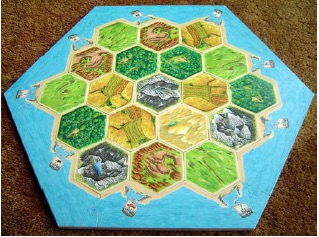
\includegraphics[width = .4\textwidth]{catan.jpg}
\end{figure}

\begin{enumerate}
  \item Is this Markov Chain irreducible? Is it aperiodic?
  \item What is the stationary distribution of this Markov Chain?
  \item Sebastian feels very safe with his ore quarry in the middle of the map. However, in the long run, what total fraction of the time will his ore quarry be occupied by the robber?
  \item Say the robber is on Sebastian's ore quarry. What is the expected amount of time it will take for the robber to return?
\end{enumerate}
\end{exercise}

\begin{solution}
\begin{enumerate}
\item Yes, the Markov Chain is irreducible because it can get from anywhere to anywhere else. The Markov Chain is also aperiodic because the robber can return back to a square in 2,3,4,5,... moves. Those numbers have a GCD of 1, so the chain is aperiodic.

\item Since this is a random walk on an undirected graph, the stationary distribution is proportional to the degree sequence. The degree for the corner pieces is 3, the degree for the edge pieces is 4, and the degree for the center pieces is 6. To normalize this degree sequence, we divide by its sum. The sum of the degrees is $6(3) + 6(4) + 7(6) = 72$. Thus the stationary probability of being on a corner is $\frac{3}{84} = \frac{1}{28}$, on an edge is $\frac{4}{84} = \frac{1}{21}$, and in the center is $\frac{6}{84} = \frac{1}{14}$.

\item From above, $\frac{1}{14}$.

\item Since this chain is irreducible and aperiodic, to get the expected time to return we can just invert the stationary probability. Thus on average it will take 14 turns for the robber to return and stop Sebastian's ore production.

\end{enumerate}
\end{solution}

\begin{exercise}
 Consider a network on the state space $1,2,...,M$, where each state represents a node within the network and the network itself is irreducible. Let $d_k$ represent the number of nodes that node $k$ connects to. Suppose we create a Markov chain as follows. At the beginning of each iteration, if the chain is at state $i$, we `'propose" to move to state $j$, where $j$ is a uniformly random selection over the nodes that $i$ is connected to. We accept this proposal and actually go to $j$ with probability min$(d_i/d_j,1)$. Find the stationary distribution of this chain.
\end{exercise}

\begin{solution}
First, we want to determine the transition matrix $Q$ for this Markov chain. Note that if we want to calculate
the probability of moving from state i to state j, we have that
$$
q_{ij} = \frac{1}{d_i}\min(d_i/d_j, 1) = \min(\frac{1}{d_j}, \frac{1}{d_i})
$$
for $i \neq j$ and nodes $i$ and $j$ are connected. $q_{ij} = 0$ otherwise.
It thus follows that $q_{ij} = q_{ji}$ for all $i, j$. Note that by the reversibility condition, $s = (s_1 , s_2 , ..., s_M )$ is stationary if $s_iq_{ij} = s_jq_{ji}$ . Since $q_{ij} = q_{ji}$ , we can choose a stationary distirbution such that all $s_i$`s are equal. It thus follows that $s_i = \frac{1}{M}$.
Thus, we can sample uniformly over all the existing state spaces by letting this Markov chain run!
\end{solution}


\begin{center}
\renewcommand{\arraystretch}{3}
\begin{tabular}{cccccc}
\textbf{Distribution} & \textbf{PDF and Support} & \textbf{EV}  & \textbf{Variance} & \textbf{MGF}\\
\hline \hline
\shortstack{Bernoulli \\ \Bern($p$)} & \shortstack{$P(X=1) = p$ \\$ P(X=0) = q$} & $p$ & $pq$ & $q + pe^t$ \\
\hline
\shortstack{Binomial \\ \Bin($n, p$)} & \shortstack{$P(X=k) = {n \choose k}p^k(1-p)^{n-k}$  \\ $k \in \{0, 1, 2, \dots n\}$}& $np$ & $npq$ & $(q + pe^t)^n$ \\
\hline
\shortstack{Geometric \\ \Geom($p$)} & \shortstack{$P(X=k) = q^kp$  \\ $k \in \{$0, 1, 2, \dots $\}$}& $q/p$ & $q/p^2$ & $\frac{p}{1-qe^t}, qe^t < 1$\\
\hline
\shortstack{Negative Binom. \\ \NBin($r, p$)} & \shortstack{$P(X=n) = {r + n - 1 \choose r -1}p^rq^n$ \\ $n \in \{$0, 1, 2, \dots $\}$} & $rq/p$ & $rq/p^2$ &  $(\frac{p}{1-qe^t})^r, qe^t < 1$\\
\hline
\shortstack{Hypergeometric \\ \Hypergeometric($w, b, n$)} & \shortstack{$P(X=k) = \sfrac{{w \choose k}{b \choose n-k}}{{w + b \choose n}}$ \\ $k \in \{0, 1, 2, \dots,  n\}$} & $\mu = \frac{nw}{b+w}$ &$\frac{w+b-n}{w+b-1}n\frac{\mu}{n}(1 - \frac{\mu}{n})$& $-$  \\
\hline
\shortstack{Poisson \\ \Pois($\lambda$)} & \shortstack{$P(X=k) = \frac{e^{-\lambda}\lambda^k}{k!}$ \\ $k \in \{$0, 1, 2, \dots $\}$} & $\lambda$ & $\lambda$ & $e^{\lambda(e^t-1)}$ \\
\hline
\hline
\shortstack{Uniform \\ \Unif($a, b$)} & \shortstack{$ f(x) = \frac{1}{b-a}$ \\$ x \in (a, b) $} & $\frac{a+b}{2}$ & $\frac{(b-a)^2}{12}$ &  $\frac{e^{tb}-e^{ta}}{t(b-a)}$\\
\hline
\shortstack{Normal \\ $\N(\mu, \sigma^2)$} & \shortstack{$f(x) = \frac{1}{\sigma \sqrt{2\pi}} e^{-\sfrac{(x - \mu)^2}{(2 \sigma^2)}}$ \\ $x \in (-\infty, \infty)$} & $\mu$  & $\sigma^2$ & $e^{t\mu + \frac{\sigma^2t^2}{2}}$\\
\hline
\shortstack{Exponential \\ $\Expo(\lambda)$} & \shortstack{$f(x) = \lambda e^{-\lambda x}$\\$ x \in (0, \infty)$} & $\sfrac{1}{\lambda}$  & $\sfrac{1}{\lambda^2}$ & $\frac{\lambda}{\lambda - t}, t < \lambda$\\
\hline
\shortstack{Gamma \\ $\Gam(a, \lambda)$} & \shortstack{$f(x) = \frac{1}{\Gamma(a)}(\lambda x)^ae^{-\lambda x}\frac{1}{x}$\\$ x \in (0, \infty)$} & $\sfrac{a}{\lambda}$  & $\sfrac{a}{\lambda^2}$ & $\left(\frac{\lambda}{\lambda - t}\right)^a, t < \lambda$\\
\hline
\shortstack{Beta \\ \Beta(a, b)} & \shortstack{$f(x) = \frac{\Gamma(a+b)}{\Gamma(a)\Gamma(b)}x^{a-1}(1-x)^{b-1}$\\$x \in (0, 1) $} & $\mu = \frac{a}{a + b}$  & $\frac{\mu(1-\mu)}{(a + b + 1)}$ & $-$\\
\hline
\shortstack{Chi-Squared \\ $\chi_n^2$} & \shortstack{$\frac{1}{2^{n/2}\Gamma(n/2)}x^{n/2 - 1}e^{-x/2}$\\$x \in (0, 1) $} & $n$  & $2n$ & $(1 - 2t)^{-n/2}, t < 1/2$\\
\hline
\hline
\shortstack{Multivar Uniform \\ A is support} & \shortstack{$f(x) = \frac{1}{|A|}$\\$  x \in A $} & $-$  & $-$ & $-$\\
\hline
\shortstack{Multinomial \\ \Mult$_k(n, \vec{p}$)} & \shortstack{$P(\vec{X} = \vec{n}) = {n \choose n_1\dots n_k}p_1^{n_1}\dots p_k^{n_k}$ \\ $n = n_1 + n_2 + \dots + n_k$} & $n\vec{p}$ & \shortstack{$\var(X_i) = np_i(1-p_i)$ \\ $\cov(X_i, X_j) = -np_ip_j$} & $\left(\sum_{i=1}^k p_ie^{t_i}\right)^n$ \\
\hline
\hline

\end{tabular}
\end{center}

\begin{tabular}{cccc}
\textbf{Cauchy-Schwarz} & \textbf{Markov} & \textbf{Chebychev} & \textbf{Jensen} \\
$|E(XY)| \leq \sqrt{E(X^2)E(Y^2)}$ &
$\displaystyle P(X \geq a) \leq \frac{E|X|}{a}$ &
$\displaystyle P(|X - \mu_X| \geq a) \leq \frac{\sigma^2_X}{a^2}$ &
$g$ convex: $E(g(X)) \geq g(E(X))$ \\
&&& $g$ concave: $E(g(X)) \leq g(E(X))$ \\
\end{tabular}

\end{document}
